\section{rigid  Class Reference}
\label{classrigid}\index{rigid@{rigid}}
Hold rigid body data, use {\bf objloader} {\rm (p.\,\pageref{classobjloader})} to load obj's. 


{\tt \#include $<$rigid.hpp$>$}

Inheritance diagram for rigid::\begin{figure}[H]
\begin{center}
\leavevmode
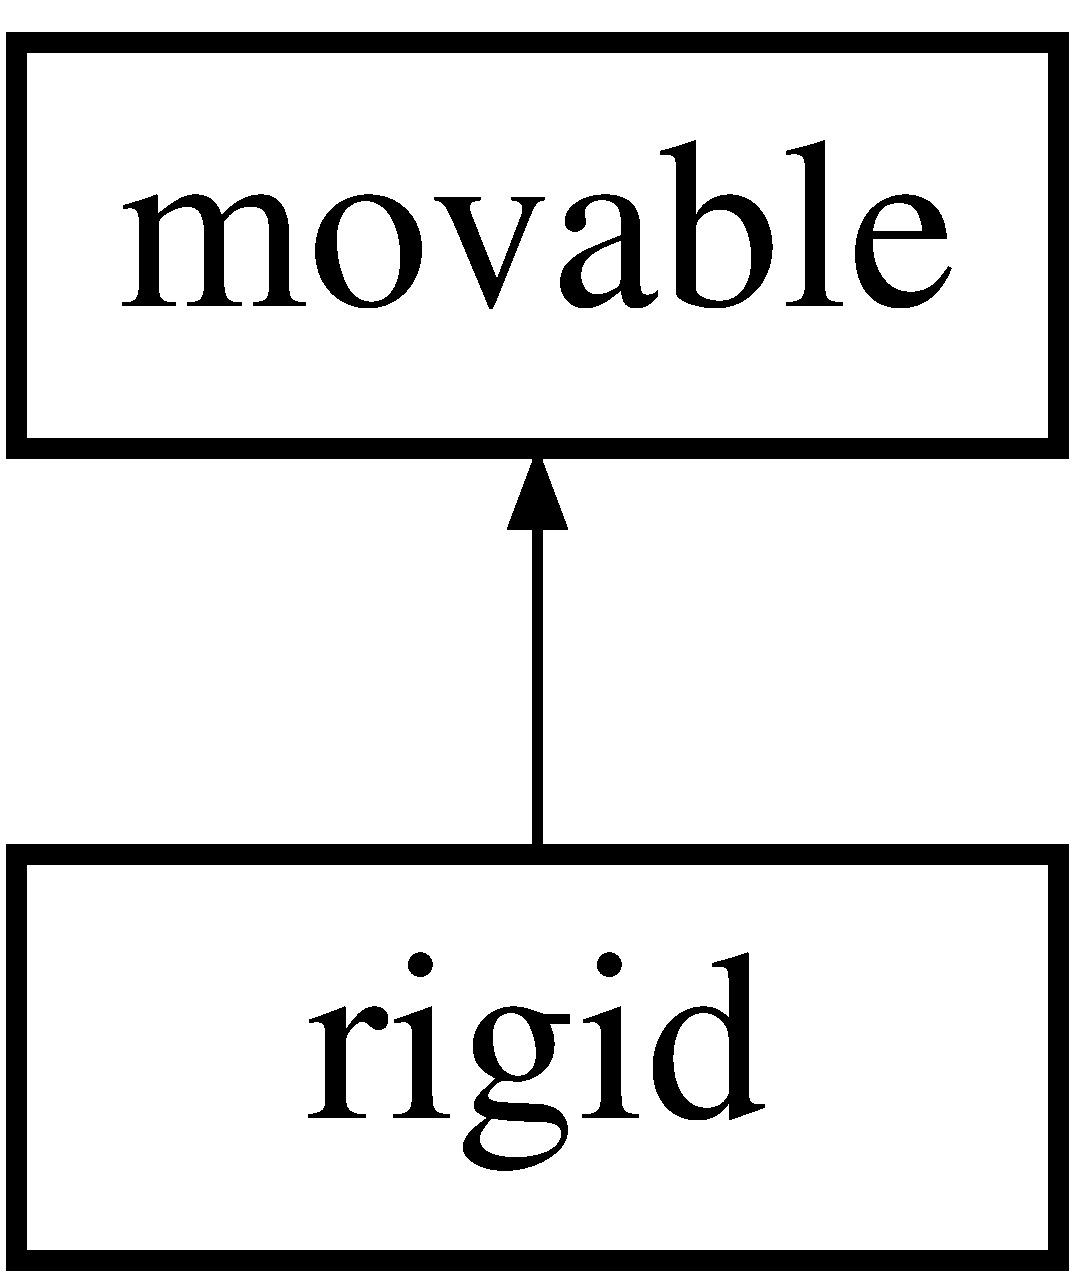
\includegraphics[height=2cm]{classrigid}
\end{center}
\end{figure}
\subsection*{Public Methods}
\begin{CompactItemize}
\item 
\index{rigid@{rigid}!rigid@{rigid}}\index{rigid@{rigid}!rigid@{rigid}}
{\bf rigid} ()\label{classrigid_a0}

\item 
\index{rigid@{rigid}!rigid@{rigid}}\index{rigid@{rigid}!rigid@{rigid}}
{\bf rigid} (string obj\-File, float STEP, string subdir)\label{classrigid_a1}

\item 
\index{~rigid@{$\sim$rigid}!rigid@{rigid}}\index{rigid@{rigid}!~rigid@{$\sim$rigid}}
{\bf $\sim$rigid} ()\label{classrigid_a2}

\item 
\index{draw@{draw}!rigid@{rigid}}\index{rigid@{rigid}!draw@{draw}}
void {\bf draw} (void)\label{classrigid_a3}

\begin{CompactList}\small\item\em Virtual generic draw member, calls make\-List.\item\end{CompactList}\item 
\index{drawDim@{drawDim}!rigid@{rigid}}\index{rigid@{rigid}!drawDim@{draw\-Dim}}
void {\bf draw\-Dim} (vector$<$ {\bf light} $\ast$ $>$ lights)\label{classrigid_a4}

\begin{CompactList}\small\item\em Adjust {\bf light} {\rm (p.\,\pageref{classlight})} intensity per-vertex.\item\end{CompactList}\item 
\index{update@{update}!rigid@{rigid}}\index{rigid@{rigid}!update@{update}}
void {\bf update} (void)\label{classrigid_a5}

\begin{CompactList}\small\item\em Does nothing currently, put scripted movements here.\item\end{CompactList}\item 
\index{makeList@{makeList}!rigid@{rigid}}\index{rigid@{rigid}!makeList@{make\-List}}
void {\bf make\-List} (void)\label{classrigid_a6}

\begin{CompactList}\small\item\em Currently not using display lists, this just draws each triangle.\item\end{CompactList}\item 
\index{getBoundingBox@{getBoundingBox}!rigid@{rigid}}\index{rigid@{rigid}!getBoundingBox@{get\-Bounding\-Box}}
void {\bf get\-Bounding\-Box} (void)\label{classrigid_a7}

\begin{CompactList}\small\item\em Virtual member that finds the extrema of all the vertices.\item\end{CompactList}\end{CompactItemize}
\subsection*{Public Attributes}
\begin{CompactItemize}
\item 
\index{counter@{counter}!rigid@{rigid}}\index{rigid@{rigid}!counter@{counter}}
int {\bf counter}\label{classrigid_m0}

\begin{CompactList}\small\item\em For scripted movements, unused currently.\item\end{CompactList}\end{CompactItemize}


\subsection{Detailed Description}
Hold rigid body data, use {\bf objloader} {\rm (p.\,\pageref{classobjloader})} to load obj's.

I thought this would be more memory efficient, to have specialized classes for loading and holding rigid body data. 



The documentation for this class was generated from the following files:\begin{CompactItemize}
\item 
{\bf rigid.hpp}\item 
rigid.cpp\end{CompactItemize}
